\chapter{Comprehensive Literature Review}
\label{ch:litreview}

Quantifying the ion energy flux delivered to a solid boundary by a bounded plasma sits at the intersection of several traditionally separate sub-disciplines: sheath/presheath theory, non-invasive electron and ion diagnostics, sputtering and erosion physics, and the statistical machinery of inverse problems and Bayesian data fusion. This chapter surveys each theme, establishes its state of the art and open controversies, and draws the threads together to motivate the framework developed later. The organisation is theme-by-theme rather than chronological, since the problem is one of synthesis and no single sub-field supplies a complete answer.

\section{Foundational Sheath and Presheath Theory}

\subsection{The Bohm Criterion: Origins and Kinetic Refinements}

The starting point for any treatment of ion energy flux is the sheath, the boundary layer that forms wherever a plasma contacts a solid surface. Because electrons are far more mobile than ions at equal temperature, the plasma develops a thin, positive layer that confines bulk electrons and accelerates ions toward the surface. The Bohm criterion requires ions to enter the sheath with a directed velocity at least equal to the Bohm speed,
\begin{equation}
u_{\mathrm{B}} = \sqrt{\frac{k_{\mathrm{B}} T_{\mathrm{e}}}{M_{\mathrm{i}}}},
\label{eq:bohm-speed}
\end{equation}
where $T_{\mathrm{e}}$ is the electron temperature and $M_{\mathrm{i}}$ the ion mass. The classical derivation combines ion continuity and energy conservation in a cold, collisionless presheath,
\begin{equation}
n_{\mathrm{i}}(x)\,u_{\mathrm{i}}(x) = n_{0}u_{0}, \qquad
\tfrac{1}{2}M_{\mathrm{i}}u_{\mathrm{i}}^{2}(x) + e\,\phi(x) = \tfrac{1}{2}M_{\mathrm{i}}u_{0}^{2},
\end{equation}
with Boltzmann-distributed electrons, $n_{\mathrm{e}}(x) = n_{0}\exp\!\big(e\phi(x)/k_{\mathrm{B}}T_{\mathrm{e}}\big)$, and Poisson's equation,
\begin{equation}
\frac{\mathrm{d}^{2}\phi}{\mathrm{d}x^{2}} = -\frac{e}{\epsilon_{0}}\big(n_{\mathrm{i}}(x) - n_{\mathrm{e}}(x)\big).
\label{ch23-eq:poisson}
\end{equation}
Expanding the right-hand side of Eq.~\eqref{ch23-eq:poisson} to first order in $\phi$ shows a monotonic space-charge solution exists only if $u_{0} \ge u_{\mathrm{B}}$, recovering Eq.~\eqref{eq:bohm-speed} as Bohm originally argued and as later placed on a rigorous kinetic footing \cite{ref0001}. The kinetic generalisation replaces the cold-fluid ion population with an arbitrary distribution $f_{\mathrm{i}}(v)$ entering the sheath edge, giving the integral form of the criterion,
\begin{equation}
\int_{0}^{\infty} \frac{f_{\mathrm{i}}(v)}{v^{2}}\,\mathrm{d}v \;\le\; \frac{n_{\mathrm{i}0} M_{\mathrm{i}}}{k_{\mathrm{B}} T_{\mathrm{e}}},
\label{eq:kinetic-bohm-review}
\end{equation}
which reduces to Eq.~\eqref{eq:bohm-speed} for a mono-energetic beam and exposes the outsized role of the low-velocity tail of $f_{\mathrm{i}}(v)$: ions barely satisfying the criterion contribute disproportionately, and a fluid estimate tracking only moments can be invalidated by that tail. How the presheath field should behave as collisionality vanishes remains disputed, including whether the criterion is an equality or an inequality.

Extensions to warm ions, multiply charged species, secondary electron emission, and non-Maxwellian electrons are well developed \cite{ref0004}, and reformulations avoiding the singular sheath-edge field in the strict Bohm limit have clarified presheath-sheath asymptotic matching \cite{ref0009}. Whether a single criterion applies universally across collisionality, magnetisation, electronegativity, and non-thermal populations remains open \cite{ref0015}.

\subsection{Presheath Structure and Collisional Effects}

The presheath is the quasi-neutral region, typically many Debye lengths in extent, over which ions accelerate from thermal bulk velocity to the Bohm speed. Its structure depends on the dominant momentum-loss mechanism: ionisation-driven presheaths in weakly ionised discharges, collision-dominated presheaths at higher pressure, and geometric presheaths set by confinement scale. Two-fluid treatments show the presheath-sheath boundary is a matter of definition rather than a sharp discontinuity \cite{ref0023}; the sheath is more properly the limit where the Debye length matches the density-gradient scale, requiring matched asymptotic expansions to connect the regions \cite{ref0013}. Collisional presheaths, where ion-neutral collisions dominate the friction against acceleration, modify the effective sheath-edge velocity and, in the fully collisional limit, replace the kinetic Bohm criterion with a fluid drift-diffusion balance \cite{ref0024}. Charge-exchange collisions reducing wall-incident ion flux have been treated as an explicit correction to the collisionless estimate \cite{ref0077}.

\subsection{Magnetised and Multi-Species Generalisations}

When a magnetic field intersects the boundary obliquely, the presheath acquires a further structure — the magnetic presheath or Chodura layer — over which ions turn from motion along the field line to motion along the density gradient, satisfying a magnetised Bohm criterion at the entrance to the Debye sheath \cite{ref0017}. This layer, of order the ion Larmor radius, sits between the electrostatic sheath and the longer collisional/ionisation presheath, giving the boundary a three-scale structure whenever the field is not normal to the surface. In multi-ion-species plasmas, individual species need not each satisfy their own marginal condition — only the species-summed criterion must hold, confirmed via laser-induced-fluorescence measurements of two ion species approaching the sheath edge together \cite{ref0329}. In electronegative and dusty plasmas, negative ions or charged dust grains modify electron screening and can shift the marginal Bohm speed from the single-species value.

\subsection{Open Questions and Controversies}

Despite more than seven decades of development since Bohm's original argument, no fully general theory of the plasma-sheath transition commands unanimous acceptance \cite{ref0015}. Disagreements persist over the sheath-edge field singularity, whether an inequality or marginal equality is physically realised in weakly collisional plasmas, the correct closure for the ion energy equation in fluid models, and how continuum-kinetic solvers should implement boundary conditions. These are not academic disputes: any attempt to quantify ion energy flux from first principles inherits them, since the flux is a moment of $f_{\mathrm{i}}(v)$ evaluated precisely where the theory is least settled.

\subsection{Model Hierarchies: Fluid, Kinetic, and Particle-Based Solution Strategies}

These disagreements reflect the fact that the sheath-presheath problem admits three distinct solution classes on different points of the accuracy-versus-cost curve, with no preferred hierarchy for coupling them. Fluid (moment) models close the ion continuity and momentum equations with an assumed equation of state, cheap enough for reactor-scale simulation but discarding the low-order velocity-space structure Eq.~\eqref{eq:kinetic-bohm-review} shows to be consequential \cite{ref0023}. Fully kinetic particle-in-cell methods retain the complete distribution function but introduce statistical noise controlled only through particle-count scaling, with explicit time-stepping tying affordable domain size to the Debye length and plasma frequency \cite{ref0631}. Continuum-kinetic solvers discretising the Vlasov equation on a phase-space grid eliminate particle noise at the cost of memory scaling unfavourably with resolved velocity-space dimensions \cite{ref0659}. Practical recipes for patching a fluid or hybrid solution to a kinetic sheath treatment offer a pragmatic middle path \cite{ref0012}. No consensus exists on which hierarchy suffices for a given accuracy target, motivating the approach adopted here: the model hierarchy itself is treated as a further source of epistemic uncertainty, quantified alongside measurement noise.

\section{Time-Varying and Radio-Frequency Sheaths}

\subsection{RF Sheath Models and Ion Transit-Time Effects}

Radio-frequency (RF) capacitively coupled plasmas present a qualitatively different sheath problem: the sheath boundary oscillates at the driving frequency (typically $\SI{13.56}{\mega\hertz}$ or a harmonic), and the ion response depends on the ratio of the RF period to the ion transit time. In the low-frequency limit ions respond quasi-statically, producing a bimodal energy distribution at the electrode; in the high-frequency limit ions respond only to the time-averaged field, producing a narrow, quasi-mono-energetic distribution \cite{ref0055}. Analytic RF sheath models — collisionless, collisional, hybrid — bridge these limits, predicting sheath voltage, thickness, and ion energy distribution versus frequency, pressure, and waveform \cite{ref0038}. The classical Child-Langmuir space-charge-limited current law for a static planar diode,
\begin{equation}
J = \frac{4}{9}\,\epsilon_{0}\sqrt{\frac{2e}{M_{\mathrm{i}}}}\,\frac{V^{3/2}}{s^{2}},
\label{ch23-eq:child-langmuir}
\end{equation}
where $V$ is the sheath voltage drop and $s$ the instantaneous sheath thickness, remains the backbone of most time-averaged RF sheath models, with $s(t)$ evolving self-consistently with the RF voltage.

\subsection{Kinetic and Particle-in-Cell Descriptions of RF Sheath Dynamics}

Because ion transit times are frequently comparable to the RF period, fully kinetic treatments are needed to capture the resulting non-Maxwellian, bimodal, or multi-modal energy distributions. Kinetic and hybrid PIC/Monte-Carlo simulations show that self-bias voltage, secondary electron emission, and waveform harmonic content all reshape the RF sheath beyond what analytic models capture \cite{ref0637}. Sawtooth and other tailored voltage waveforms control the harmonic content of the sheath modulation and hence the resulting IEDF \cite{ref0043}. Kinetic simulations of the intermediate-frequency regime have quantified how the IEDF transitions continuously between the bimodal and narrow limits \cite{ref0040}.

\subsection{Electrical Asymmetry and Ion Energy Control}

A major practical development is the deliberate exploitation of waveform tailoring to decouple ion flux and ion energy at a substrate, historically impossible in a single-frequency discharge \cite{ref0105}. The electrical asymmetry effect, whereby a phase-shifted dual- or multi-frequency waveform breaks the powered/grounded electrode symmetry, produces a DC self-bias tunable to shift mean ion energy while approximately preserving flux \cite{ref0106}, underlying essentially all modern "tailored ion energy distribution" process technology \cite{ref0105}. This body of work is almost entirely oriented toward control — producing a desired IEDF at a substrate — rather than toward inferring delivered energy flux from external, non-invasive measurements.

\section{Ion Energy Flux at Plasma Boundaries}

\subsection{Definition and the Governing Flux Integral}

The central quantity throughout this monograph is the ion energy flux delivered to a surface, the third velocity moment of the ion distribution at the sheath-plasma boundary,
\begin{equation}
\Gamma_{E} = \int_{0}^{\infty} \tfrac{1}{2} M_{\mathrm{i}} v^{2}\, v\, f_{\mathrm{i}}(v)\,\mathrm{d}v ,
\label{ch23-eq:energy-flux-def}
\end{equation}
with units of power per unit area. For a cold-ion presheath entering at exactly the Bohm speed and accelerated through the sheath drop $\Delta V_{\mathrm{sh}}$, Eq.~\eqref{ch23-eq:energy-flux-def} reduces to the engineering form,
\begin{equation}
\Gamma_{E} \approx \Gamma_{\mathrm{i}}\Big(\tfrac{1}{2}k_{\mathrm{B}}T_{\mathrm{e}} + e\,\Delta V_{\mathrm{sh}}\Big), \qquad \Gamma_{\mathrm{i}} = n_{\mathrm{s}} u_{\mathrm{B}},
\label{eq:energy-flux-eng}
\end{equation}
where $n_{\mathrm{s}}$ is the sheath-edge ion density and $\Gamma_{\mathrm{i}}$ the particle flux; the $\tfrac{1}{2}k_{\mathrm{B}}T_{\mathrm{e}}$ term reflects presheath-acquired energy, while $e\,\Delta V_{\mathrm{sh}}$ dominates for typical sheath voltages several times $T_{\mathrm{e}}$ in electron-volts. Equation~\eqref{eq:energy-flux-eng} presumes a mono-energetic, collisionless, single-species traversal — routinely violated — and prior knowledge of $n_{\mathrm{s}}$, $T_{\mathrm{e}}$, and $\Delta V_{\mathrm{sh}}$, each a diagnostic challenge in itself. Fluid models carrying the full ion energy spectrum through the sheath capture how a broadened or bimodal edge distribution propagates into the delivered flux \cite{ref0083}, and non-Maxwellian generalisations have been derived for Kappa-distributed electrons relevant to space plasmas \cite{ref0090}.

\subsection{Sensors and In Situ Flux Measurement}

Because Eq.~\eqref{ch23-eq:energy-flux-def} cannot generally be evaluated from first principles with process- or lifetime-relevant accuracy, dedicated flux sensors have been developed to measure $\Gamma_{E}$ directly, typically via a thermally isolated collector whose temperature rise is calibrated against incident power flux \cite{ref0075}, related to heat-flux microsensors for calorimetric measurement of interaction power density \cite{ref0175}. In plasma immersion ion implantation, sheath-accelerated secondary electron currents serve as a non-invasive proxy for instantaneous ion flux \cite{ref0078}. Direct wafer-surface heat-flux measurements during reactive-ion-etch processing provide a further empirical benchmark \cite{ref0080}. A consistent theme emerges: every practical sensor perturbs the plasma, is restricted to a specific geometry or waveform, or returns an integrated, energy-unresolved quantity.

\subsection{Collisional and Non-Maxwellian Corrections to the Flux}

Realistic sheaths are neither perfectly collisionless nor Maxwellian, and both departures modify Eq.~\eqref{eq:energy-flux-eng} substantially. Ion-neutral collisions broaden and skew the arriving ion energy distribution, captured in fluid and hybrid sheath models tracking the full spectrum rather than assuming ballistic acceleration \cite{ref0074}. Magnetised sheaths make delivered ion energy depend on the field-surface angle, since only the field-aligned velocity component is accelerated \cite{ref0088}. Data-driven closures for sheath heat flux, extracted from kinetic simulation data via symbolic regression, suggest the fluid-closure problem may be tractable empirically \cite{ref0101}. System-level power-balance accounting in fusion plasmas illustrates the stakes of an accurate flux estimate at reactor-engineering level \cite{ref0093}.

\section{Ion Energy Distribution Functions}

\subsection{Analytic and Numerical IEDF Models}

The ion energy distribution function (IEDF), $f_{\mathrm{i}}(E)$, is the full energy-resolved generalisation of the flux integral of Eq.~\eqref{ch23-eq:energy-flux-def}, connecting sheath theory to both diagnostics and materials response, since sputtering yield is itself strongly energy-dependent. In the collisionless, single-frequency RF limit, the IEDF at the powered electrode takes a bimodal "saddle" shape, with peaks at $E_{\min}$ and $E_{\max}$ separated by an amount scaling inversely with driving frequency and ion transit time: longer transit relative to the RF period narrows rather than widens the spread. The low-energy peak corresponds to ions near the minimum instantaneous sheath voltage during transit, the high-energy peak to those near the maximum \cite{ref0123}, generalised since to arbitrary driving frequency and Kappa-distributed suprathermal electrons \cite{ref0123}. A rigorous kinetic boundary condition connecting the bulk ion velocity distribution to fluid moments replaces the ad hoc mono-energetic assumption in most fluid models \cite{ref0119}.

\subsection{Diagnostic Reconstruction of the IEDF}

Because $f_{\mathrm{i}}(E)$ cannot generally be measured directly at the sheath edge, indirect reconstruction strategies dominate. Retarding field energy analysers (RFEAs), measuring current transmitted through biased grids versus retarding potential, remain the most widely deployed direct IEDF technique, including through RF- or pulse-biased sheaths where the response must be synchronised to the drive waveform \cite{ref0540}. Planar laser-induced-fluorescence systems extend this to a full two-dimensional spatial map \cite{ref0304}. In electric propulsion, ion energy diagnostics of the Hall-thruster exhaust plume make the IEDF a mission-critical quantity governing thrust efficiency and erosion risk \cite{ref0114}, situated within its principal application by the broader ion-thruster review \cite{ref0115}.

\section{Sputtering, Erosion, and Surface Yield Physics}

\subsection{Binary-Collision Theory and Empirical Yield Laws}

The ion energy flux delivered to a surface, quantified via Eqs.~\eqref{ch23-eq:energy-flux-def}--\eqref{eq:energy-flux-eng}, matters because it drives physical sputtering: ejection of surface atoms via momentum transfer from incident ions. The theoretical foundation is linear-cascade binary-collision theory, in which an incident ion transfers momentum through a cascade of elastic nuclear collisions, a fraction of which reach the surface with enough outward momentum to overcome the binding energy \cite{ref0143}, yielding the Sigmund sputtering-yield formula, which for normal incidence and energies well above threshold takes the form
\begin{equation}
Y(E) = \Lambda\, S_{\mathrm{n}}(E),
\end{equation}
where $\Lambda$ is a materials constant proportional to the inverse surface binding energy and $S_{\mathrm{n}}(E)$ the nuclear stopping cross section, expressible through the reduced (Lindhard) energy $\varepsilon$. The Bohdansky formula introduces a threshold energy $E_{\mathrm{th}}$ below which sputtering vanishes, reproducing the low-energy roll-off,
\begin{equation}
Y(E) = Q\, S_{\mathrm{n}}(\varepsilon) \left[1 - \left(\frac{E_{\mathrm{th}}}{E}\right)^{2/3}\right]\left[1 - \frac{E_{\mathrm{th}}}{E}\right]^{2},
\label{ch23-eq:bohdansky}
\end{equation}
with $Q$ a target-dependent constant, illustrated schematically in Fig.~\ref{fig:sputter-yield}. Direct experimental sputtering-yield measurements under controlled ion-beam and plasma bombardment \cite{ref0152} remain the principal calibration source for $\Lambda$, $Q$, and $E_{\mathrm{th}}$, and comprehensive treatments of the collision-cascade physics remain the reference framework for newer molecular-dynamics and machine-learning yield models \cite{ref0144}. The single-parameter yield curve is at best leading-order; energy- and angle-resolved sputtering, driven by the full IEDF rather than a single characteristic energy, is the physically correct generalisation and precisely the coupling this monograph seeks to exploit.

\begin{figure}[htbp]
\centering
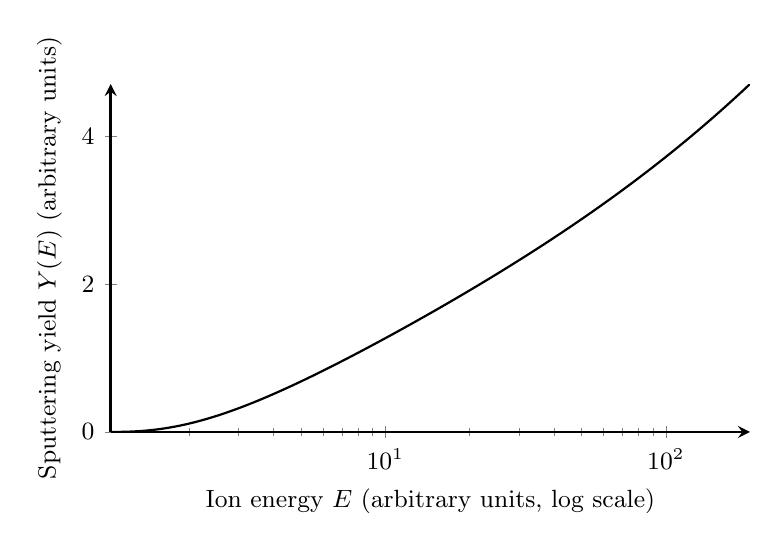
\begin{tikzpicture}
\begin{axis}[
 width=0.8\linewidth, height=6cm,
 xlabel={Ion energy $E$ (arbitrary units, log scale)},
 ylabel={Sputtering yield $Y(E)$ (arbitrary units)},
 xmode=log,
 domain=1.05:200,
 samples=200,
 axis lines=left,
 grid=none,
 line width=0.9pt,
 every axis plot/.append style={color=black},
 tick label style={font=\small},
 label style={font=\small},
]
\addplot[black, thick] { (1 - (1/x)^(2/3)) * (1 - 1/x)^2 * (x^0.3) };
\end{axis}
\end{tikzpicture}
\caption{Schematic, illustrative plot of the analytic Bohdansky-type sputtering-yield law of Eq.~\eqref{ch23-eq:bohdansky}, normalised to a unit threshold energy $E_{\mathrm{th}}=1$ and plotted against a simplified power-law stand-in for the nuclear stopping cross section $S_{\mathrm{n}}(\varepsilon)\propto E^{0.3}$. The curve illustrates the functional form only and does not represent measured or fitted data for any specific ion-target combination.}
\label{fig:sputter-yield}
\end{figure}

\subsection{Erosion Measurement and Long-Term Lifetime Assessment}

Translating an instantaneous sputtering yield into cumulative erosion depth or mass-loss rate requires integrating it against the full, time-dependent, energy- and angle-resolved ion flux over a component's operational lifetime — a direct application of the problem addressed here. In fusion plasma-facing-component research, the gross and net erosion balance of tungsten and other divertor materials has been measured and modelled extensively \cite{ref0158}, and dedicated material-testing facilities expose candidates to controlled ion energy fluxes for erosion-rate calibration \cite{ref0586}. Comparisons of predicted erosion, using yield laws such as Eq.~\eqref{ch23-eq:bohdansky}, against measured erosion of tungsten coatings reveal discrepancies from redeposition, morphology evolution, and mixed-species bombardment not captured by the flat-surface formula \cite{ref0593}. In electric propulsion, channel-wall erosion in Hall-effect thrusters, driven by near-wall sheath impact on the ceramic discharge channel, has been measured directly via laser-induced fluorescence of sputtered wall material \cite{ref0454} and reviewed as the principal life-limiting mechanism for this thruster class \cite{ref0440}. Surface characterisation techniques — interferometry, thickness measurement, witness-coating methods — offer post-exposure routes trading resolution against invasiveness. The gap mirrors that for flux sensing: erosion measurement is almost universally destructive/post-hoc, motivating a forward-predictive alternative.

\section{Plasma-Material Interaction and Heat Flux}

The ion energy flux problem generalises to total power deposition — ion kinetic energy, recombination energy, and electron heat flux combined — onto a plasma-facing surface. High-heat-flux plasma-material interaction has been studied intensively in fusion, where transient events such as edge-localised modes and disruptions deposit power densities orders of magnitude above steady state, driving melt-layer formation, cracking, and rapid material loss on tungsten and molybdenum components \cite{ref0581}. Physical modelling of the resulting vapour-shielding effect, where ablated material absorbs and re-radiates incident heat flux, illustrates the strongly nonlinear, self-limiting character of extreme plasma-material interaction \cite{ref0176}. Materials-screening studies rank candidates against combined erosion and heat-flux-tolerance criteria \cite{ref0189}, while broader reviews treat the two as jointly limiting constraints \cite{ref0190}. Diagnostics here include direct heat-flux microsensors \cite{ref0175} and laser Thomson scattering adapted for divertor and limiter edge plasmas \cite{ref0383}.

\section{Electrostatic Probe Diagnostics}

Langmuir probes remain the most widely deployed diagnostic for local electron temperature and density in low-temperature and processing plasmas, feeding directly into the Bohm-speed and sheath-voltage estimates of Eq.~\eqref{eq:energy-flux-eng}. The classical single-probe I-V characteristic analysis, extracting electron temperature from the semi-logarithmic slope of the electron-retarding-region current, has been refined through fitting procedures reducing sensitivity to probe contamination, RF pickup, and non-Maxwellian distortion \cite{ref0217}. Gyrofluid-simulation-based analyses of probe-measured temperatures quantify biases inherent to the fluid interpretation of probe traces \cite{ref0194}. Comparisons of Langmuir-probe-derived $T_{\mathrm{e}}$ and $n_{\mathrm{e}}$ against OES \cite{ref0237} and Thomson scattering \cite{ref0355} provide essential cross-validation, though systematic offsets persist in magnetised or strongly non-Maxwellian plasmas. In the fusion-edge context, Langmuir-probe arrays remain the primary means of characterising the electron energy distribution and plasma potential at the tokamak boundary \cite{ref0213}. A recommended-practice document for electric-propulsion testing codifies probe construction, sweep circuitry, and data interpretation for thruster plasmas \cite{ref0226}.

\section{Optical Emission Spectroscopy and Collisional-Radiative Modeling}

Optical emission spectroscopy (OES) offers a non-invasive alternative to probe-based diagnostics, inferring electron temperature and density from relative intensities of atomic or ionic emission lines. Because excited-state populations are set by a balance of excitation, de-excitation, ionisation, and radiative decay, quantitative interpretation of OES line ratios requires a collisional-radiative (CR) model rather than a corona- or LTE-equilibrium assumption \cite{ref0260}. Line-ratio methods based on helium metastable and resonance transitions are a well-validated CR-model application, cross-checked against probe and Thomson-scattering measurements \cite{ref0266}. Argon CR models have received sustained development given argon's ubiquity as a processing gas \cite{ref0245}, including Bayesian frameworks propagating atomic-data uncertainty through to inferred $T_{\mathrm{e}}$ and $n_{\mathrm{e}}$ \cite{ref0275}.

OES has also extracted time-resolved electron temperature evolution in Hall thrusters synchronised to discharge oscillations \cite{ref0256}. Tomographic reconstruction of the spatially resolved electron-property field from line-integrated OES chords has been demonstrated for the Hall-thruster acceleration region \cite{ref0257}. Real-time OES-based process monitoring has become standard for closed-loop control of deposition and etch processes \cite{ref0553}.

\section{Laser-Induced Fluorescence and Ion Velocity Distribution Function Measurement}

Laser-induced fluorescence (LIF) occupies a uniquely important position because, unlike OES or Langmuir probes, it provides a non-invasive, spatially and spectrally resolved measurement of the ion velocity distribution function itself, not only its low-order moments. A narrow-linewidth tunable laser is scanned across a Doppler-broadened absorption transition of a metastable ion state, and fluorescence intensity versus detuning maps the projection of $f_{\mathrm{i}}(v)$ along the laser direction \cite{ref0292}, applied extensively to characterise ion dynamics near the sheath boundary \cite{ref0329} and providing the most direct experimental window onto the kinetic quantities entering Eq.~\eqref{eq:kinetic-bohm-review} and Eq.~\eqref{ch23-eq:energy-flux-def}. Planar and tomographic LIF implementations extend the single-point measurement to a full multi-dimensional map, of particular value in electric-propulsion plumes \cite{ref0328}.

Within electric propulsion, LIF has become the diagnostic of record for ion velocity distributions in Hall-thruster channels and plumes, revealing multi-population structure — counter-streaming and near-wall populations — invisible to bulk flux or probe measurements \cite{ref0322}. Comprehensive reviews of the LIF technique provide the methodological foundation this monograph builds on \cite{ref0347}.

\section{Thomson Scattering and Interferometric Density Diagnostics}

Incoherent Thomson scattering provides a first-principles, calibration-independent measurement of the local electron velocity distribution, and hence $T_{\mathrm{e}}$ and $n_{\mathrm{e}}$, through the Doppler broadening and intensity of light scattered from free electrons by an intense probe laser \cite{ref0354}. Its principal limitation — an extremely small scattering cross section requiring high electron density or a very high-power laser — has been addressed through portable, temporally resolved systems for low-density plasmas \cite{ref0357}, and spatially resolved implementations mapping electron properties across a magnetically shielded Hall thruster's acceleration region \cite{ref0356}. Because it measures the electron distribution directly without an atomic model, Thomson scattering provides an independent cross-check against Langmuir-probe and OES/CR-model-derived properties \cite{ref0355}; comparisons across all three quantify the achievable agreement and residual discrepancies from probe perturbation or atomic-data uncertainty.

Microwave and laser interferometry complement Thomson scattering with a line-integrated but simple, robust electron-density measurement via the plasma-induced phase shift of a probe beam. Multi-chord configurations enable coarse tomographic resolution of the density profile \cite{ref0399}, valuable for the fusion-edge profiles discussed later. Dispersion-interferometer configurations, suppressing sensitivity to vibration and beam steering by combining two harmonically related probe frequencies, have been deployed in pulsed-power and transmission-line contexts requiring high time resolution \cite{ref0417}.

\section{Electric Propulsion: Erosion and Diagnostics of Hall and Ion Thrusters}

Electric propulsion is one of the most demanding, thoroughly instrumented application domains for ion energy flux quantification, since Hall-effect and gridded ion thrusters rely on a confined sheath to accelerate ions, and both suffer life-limiting erosion driven by the ion energy flux incident on discharge-channel walls or accelerator grids. In Hall thrusters, near-wall ion bombardment of the ceramic discharge channel is the dominant erosion mechanism, and two-dimensional hybrid and fully kinetic PIC models predict erosion rates and lifetime from first principles \cite{ref0433}. Reviews of Hall-thruster erosion synthesise decades of experience, from empirical scaling laws to self-consistent kinetic prediction \cite{ref0440}. Magnetic shielding — deflecting the bulk of the energetic ion flux away from the channel wall — has transformed erosion-limited lifetime, and near-wall transport in shielded configurations continues to be studied \cite{ref0425}. In gridded ion thrusters, accelerator-grid erosion driven by charge-exchange bombardment, rather than direct beam-ion impact, has been modelled using dedicated plume codes validated against measured patterns \cite{ref0463}.

Diagnostic methodology specific to electric propulsion has matured into its own recommended-practice literature, spanning Langmuir and emissive probe protocols \cite{ref0226}, RFEA design for plume ion-energy characterisation \cite{ref0490}, and reviews of the instrumentation suite for ground-test and in-flight packages \cite{ref0506}. A well-documented complication is facility background-gas pressure, which introduces charge-exchange pathways absent in space and biases measured performance and erosion \cite{ref0461} — a practical manifestation of the same collisional-correction issue treated theoretically above.

\section{Plasma Etching and Semiconductor Process Diagnostics}

Reactive-ion and plasma etching depend critically on the ion energy delivered to the wafer surface, since etch rate, selectivity, and profile anisotropy are strongly and often non-monotonically dependent on the incident ion energy distribution. Model-based coupling of ion energy flux to spatially resolved etch-profile evolution, convolving the local angle- and energy-dependent etch yield with evolving surface topography, has been developed for collisionless sheaths typical of low-pressure etch tools \cite{ref0074}. Foundational reviews of plasma etching technology situate the problem within the semiconductor-manufacturing context, covering etch mechanisms, mask selectivity, and the etch-rate/anisotropy trade-off \cite{ref0536}. Independent control of ion density and bombardment energy — via dual-frequency schemes related to the electrical-asymmetry techniques above — remains a central goal of process-tool design, since selectivity and damage thresholds impose conflicting constraints on the acceptable energy window \cite{ref0539}.

Complementary in situ diagnostics include broader treatments of plasma diagnostics for real-time monitoring and closed-loop control \cite{ref0553}. Direct measurement of the ion energy distribution using retarding-potential analysers, in RF and pulsed-DC configurations, provides the empirical benchmark for the model-based predictions above \cite{ref0540}. Despite its maturity and commercial stakes, this literature remains largely tool- and recipe-specific; a generalisable framework transferring across chemistries and geometries is an opportunity this monograph addresses.

\section{Fusion Plasma-Wall Interaction and the Tokamak Edge}

The scrape-off layer (SOL) and divertor regions of a magnetically confined fusion device present perhaps the most consequential real-world instance of the ion-energy-flux problem, since divertor heat and particle flux directly govern component lifetime and, at reactor scale, the feasibility of steady-state operation. The SOL heat-flux width — the radial decay length over which heat flux is deposited onto the divertor target — is the subject of intensive multi-machine scaling studies and continued controversy over extrapolation to reactor parameters. Power-deposition models spanning simple convective formulations through to turbulence simulations resolving divertor heat load during thermal-quench transients illustrate the same fluid-versus-kinetic tension already encountered in sheath theory, now at tokamak-engineering scale \cite{ref0605}. High-heat-flux testing facilities reproducing ITER-relevant divertor loading on candidate mock-ups provide the essential validation layer \cite{ref0581}.

SOL turbulence — intermittent, filamentary blob transport dominating cross-field transport near the SOL — has been characterised through gyrokinetic and reduced fluid simulation \cite{ref0605} and through direct filament tracking using fast visible imaging and probe arrays on MAST and Alcator C-Mod \cite{ref0600}. RFEA measurements of ion temperature at the divertor target provide one of the few direct, energy-resolved constraints on the flux actually delivered to a tokamak surface, rather than inferred via upstream measurements and a sheath-transmission model \cite{ref0610}.

\section{Kinetic Theory and Particle-in-Cell Simulation of the Sheath}

Fully kinetic simulation, whether via Lagrangian particle-in-cell (PIC) methods or Eulerian continuum-kinetic (Vlasov) solvers, provides the most rigorous route to computing $f_{\mathrm{i}}(v)$ self-consistently across the presheath-sheath system without invoking fluid closure assumptions. The original fully kinetic, self-consistent PIC treatment of the collisionless plasma-sheath region established the basic simulation methodology still in wide use, resolving the sheath potential profile, ion velocity distribution, and Bohm-criterion satisfaction from first principles \cite{ref0631}. Subsequent PIC studies have extended this to magnetised sheaths \cite{ref0633} and ion-ion (electronegative or dual-species) sheath and presheath structure \cite{ref0655}. Continuum-kinetic (Eulerian, discontinuous-Galerkin) solvers, discretising the Vlasov equation on a phase-space grid rather than sampling with finite-weight particles, eliminate PIC's statistical noise at the cost of substantially higher computational and memory demand, and have resolved fine structure in the sheath-edge ion distribution — including the low-velocity tail central to Eq.~\eqref{eq:kinetic-bohm-review} — with a fidelity difficult for particle methods \cite{ref0659}. The Tonks-Langmuir model — an exactly solvable, ionisation-dominated kinetic presheath model — remains the canonical benchmark for numerical kinetic solvers, and continued debate over whether the kinetic Bohm criterion is an assumption or a derivable theorem within it shows that even this idealised problem retains open questions \cite{ref0665,ref0666}.

\section{Inverse Problems, Bayesian Inference, and Multi-Diagnostic Data Fusion}

The final theme is methodological rather than purely physical: reconstructing an underlying quantity — the sheath-edge ion energy distribution or the delivered energy flux — from indirect, noisy, incomplete measurements. Classical regularisation theory, most prominently Tikhonov regularisation, stabilises the otherwise ill-posed inversion of a convolved measurement back to the underlying resolved quantity, applied to tomographic laser-absorption spectroscopy problems structurally analogous to plasma-diagnostic tomography \cite{ref0677}. Related strategies — total-variation penalisation, iterative regularisation, and regularisation-parameter selection — have been developed across imaging and spectroscopy inverse problems \cite{ref0692}, a mature toolkit transferable to plasma-diagnostic inversion. Optical tomography of plasma emission, reconstructing a spatially resolved emissivity field from limited chordal measurements, is a direct instance of the same ill-posed problem, addressed through both classical algebraic reconstruction and Bayesian tomographic frameworks \cite{ref0685}.

Bayesian inference has emerged as the dominant modern methodology for principled multi-diagnostic data fusion in plasma physics, treating each diagnostic as an imperfect, noisy observation of a shared plasma state combined through a rigorously specified joint likelihood and prior \cite{ref0706}. Integrated data analysis frameworks of this type have been deployed extensively at major tokamak facilities, fusing Thomson scattering, interferometry, and magnetic equilibrium reconstruction into a single self-consistent kinetic-profile inference for ITER operation \cite{ref0706}, and comprehensive reviews catalogue both the methodology's successes and its remaining computational-cost and prior-specification challenges \cite{ref0710}. Bayesian model selection has been applied to Thomson-scattering spectral analysis to discriminate between competing models on a rigorous statistical footing rather than by visual inspection \cite{ref0684}, and analogous frameworks have been applied to combined OES/CR-model inference, propagating atomic-data uncertainty through to inferred electron properties \cite{ref0275}. In electric propulsion, Bayesian calibration and uncertainty quantification of Hall-thruster models against multi-diagnostic measurement sets illustrates this methodology's applicability to the erosion- and flux-relevant problems above \cite{ref0719}. The broader review of data-driven plasma science underscores the growing consensus that principled uncertainty quantification, rather than point-estimate reporting, should be the standard for any inferred plasma quantity \cite{ref0711}.

\section{Synthesis: Cross-Theme Connections to the Proposed Framework}

Read individually, the fifteen themes surveyed above appear as largely independent literatures, each with its own journals and vocabulary. Read together, a single connected chain becomes visible, and it is this chain the framework developed in this monograph seeks to instantiate end to end. Sheath and presheath theory supplies the first-principles relationship between bulk-plasma parameters ($T_{\mathrm{e}}$, $n_{\mathrm{e}}$, $f_{\mathrm{i}}(v)$) and the sheath-edge ion flux and energy, formalised in the Bohm criterion of Eq.~\eqref{eq:bohm-speed} and its kinetic generalisation, Eq.~\eqref{eq:kinetic-bohm-review}. Time-varying and RF sheath theory extends this to the driven boundary conditions of essentially all technologically deployed plasmas, introducing the Child-Langmuir scaling of Eq.~\eqref{ch23-eq:child-langmuir} and the bimodal IEDF structure. The ion-energy-flux and IEDF literatures then define the target quantity itself — Eqs.~\eqref{ch23-eq:energy-flux-def}--\eqref{eq:energy-flux-eng} — and expose the central practical difficulty: existing sensors either perturb the measurement, are geometry- or waveform-specific, or return only an energy-integrated quantity.

The diagnostic themes — electrostatic probes, OES/CR modelling, laser-induced fluorescence, and Thomson scattering/interferometry — supply the raw, non-invasive observables from which the bulk-plasma inputs to the sheath theory can be reconstructed. Each measures a different moment of the underlying plasma state, with its own noise, resolution, and systematic-error structure; the sustained cross-comparison literature between the three documents both the value and the limits of any single diagnostic in isolation. This is precisely the gap the inverse-problems and data-fusion literature closes: rigorous, uncertainty-aware combination of multiple imperfect channels into a single, self-consistent estimate of the plasma state and, via the sheath theory above, of the ion energy flux itself.

The consequences of an accurately quantified flux are made concrete by the applied themes: sputtering and erosion physics, translating the flux into a materials-lifetime prediction via yield laws such as Eq.~\eqref{ch23-eq:bohdansky}; plasma-material interaction, extending the same accounting to total power deposition; and the three application domains — electric propulsion, semiconductor etching, and fusion plasma-wall interaction — each of which, largely without cross-fertilisation, has developed its own methodology built on an incomplete or facility-specific flux estimate. Kinetic theory and PIC simulation provide the ground truth against which any reduced, diagnostic-driven framework must ultimately be validated, closing the loop back to the sheath physics with which this review began.

A second, orthogonal axis concerns measurement philosophy: invasiveness, and whether a technique returns a full energy-resolved distribution (as LIF and retarding-field analysis do) or only a low-order moment (as interferometry and single-point Langmuir sweeps do). No single technique is simultaneously non-invasive and fully energy-resolved at an arbitrary surface: LIF requires seeding a metastable ion state and optical access rarely available on an operational component; Thomson scattering is non-invasive but measures electrons, requiring the sheath theory above to translate that into an ion-flux inference; retarding-field analysis is fully energy-resolved but unavoidably invasive. This is why multi-diagnostic data fusion is a structural necessity: non-invasiveness, full energy resolution, and applicability to an arbitrary surface are individually available but never jointly available in one instrument, and only a fusion of complementary measurements, propagated through the sheath-theoretic forward model, can recover all three.

A third connecting thread is the shared mathematical structure of the forward problem across all three applied domains. The practically consequential quantity is not the flux at a single instant or point, but its integral over an operational lifetime and the full illuminated surface — a cumulative erosion depth, etch profile, or divertor thermal fatigue load. Because the underlying yield and heat-deposition functions (Eq.~\eqref{ch23-eq:bohdansky} and its generalisations) are strongly nonlinear in instantaneous ion energy, this cumulative quantity cannot be obtained correctly from a single averaged flux estimate; it requires the full, resolved energy distribution integrated through the nonlinear yield law. This is elevated to a first-class design requirement here: any acceptable solution must deliver the full distribution $f_{\mathrm{i}}(E)$, not merely its low-order moments, because the downstream engineering quantities are nonlinear functionals of that distribution.

\section{The Gap This Work Fills}

Three specific, interlocking gaps emerge from this synthesis. First, no existing sheath-theory or IEDF model is routinely coupled to a multi-diagnostic Bayesian inference layer capable of ingesting realistically available non-invasive observables and returning an energy-resolved, uncertainty-quantified estimate of $f_{\mathrm{i}}(E)$ and $\Gamma_{E}$; the sheath-theory and data-fusion literatures, though individually mature, have developed largely in parallel. Second, existing ion-energy-flux sensors and erosion-measurement techniques are almost without exception invasive, geometry-specific, energy-integrated, or restricted to post-hoc/destructive analysis, leaving a clear opening for a model-based, forward-predictive alternative. Third, the applied communities that most urgently need accurate flux quantification — electric propulsion, semiconductor processing, and fusion plasma-wall interaction — have each developed self-contained, domain-specific methodologies with limited cross-transfer, despite facing an identical underlying inference problem. The framework developed in the chapters that follow addresses all three simultaneously: it couples kinetic sheath theory to a principled Bayesian inversion, targets the full energy-resolved flux rather than an integrated proxy, and generalises across the three applied domains.

\section{Summary}

This chapter has surveyed fifteen interlocking research themes spanning the theoretical, diagnostic, and applied literature relevant to quantifying ion energy flux across plasma sheaths. Table~\ref{tab:theme-maturity} summarises each theme together with a qualitative assessment of its maturity and relevance to the framework developed here. The overarching conclusion is that while the individual building blocks — kinetic sheath theory, non-invasive diagnostics, sputtering and erosion physics, and Bayesian data fusion — are each independently mature, their integration into a single, generalisable, energy-resolved, uncertainty-quantified flux-estimation pipeline remains unrealised. Closing this integration gap is what the remainder of this monograph is devoted to.

\begin{table}[htbp]
\centering
\caption{Summary of the research themes surveyed in this chapter, their approximate scientific maturity, and their principal relevance to the ion-energy-flux quantification framework developed here. Maturity ratings are qualitative judgments by the authors, not a bibliometric score.}
\label{tab:theme-maturity}
\begin{tabularx}{\linewidth}{@{}l l X@{}}
\toprule
\textbf{Theme} & \textbf{Maturity} & \textbf{Principal relevance to this work} \\
\midrule
Sheath/presheath theory, Bohm criterion & Mature, open edges & Governing relation between bulk plasma and boundary flux \\
RF and time-varying sheaths & Mature & Driven-boundary condition; bimodal IEDF origin \\
Ion energy flux quantification & Emerging & Target quantity; existing sensors invasive/limited \\
Ion energy distribution functions (IEDF) & Mature & Full energy-resolved generalisation of the flux \\
Sputtering and erosion yield physics & Mature & Converts flux into materials-lifetime prediction \\
Plasma-material interaction / heat flux & Mature & Extends flux accounting to total power deposition \\
Electrostatic (Langmuir) probes & Mature & Invasive bulk-plasma input diagnostic \\
OES and collisional-radiative modelling & Mature & Non-invasive electron-property diagnostic \\
Laser-induced fluorescence / IVDF & Mature & Direct, non-invasive $f_{\mathrm{i}}(v)$ measurement \\
Thomson scattering / interferometry & Mature & First-principles, cross-validating diagnostics \\
Electric propulsion erosion \& diagnostics & Mature, applied & Primary applied domain; lifetime-critical \\
Plasma etching / semiconductor diagnostics & Mature, applied & Second applied domain; process-critical \\
Fusion plasma-wall interaction / SOL & Mature, applied & Third applied domain; reactor-critical \\
Kinetic theory / PIC simulation & Mature & First-principles validation ground truth \\
Inverse problems / Bayesian data fusion & Emerging in plasma physics & Methodological bridge closing the integration gap \\
\bottomrule
\end{tabularx}
\end{table}
